\documentclass[aspectratio=169, xcolor={table}]{beamer}

\usepackage[utf8]{inputenc}
\usepackage[T1]{fontenc}
\usepackage[brazil]{babel}
\usepackage{graphicx}
\usepackage{amsmath}
\usepackage{booktabs}

% Configuração do Tema
\usetheme{Madrid}
\usecolortheme{whale}

% Informações do Título
\title[ASCM - Limpeza e Arrefecimento]{Sistema Automatizado de Limpeza e Arrefecimento de Painéis Fotovoltaicos (ASCM)}
\subtitle{Proposta de Projeto Integrado - Engenharia de Controle e Automação}
\author[César, Lucas, Paulo]{
    Equipe: \\
    César Kerber, Lucas Ekroth, Paulo Rangel
}
\institute[IFSP]{
    \textbf{Orientador:} Prof. Valdeci Donizete Gonçalves \\
}
\date{\today}

\begin{document}

% Slide de Título
\begin{frame}
    \titlepage
\end{frame}


% --- Introdução e Motivação ---
\section{Introdução e Motivação}

\begin{frame}{Contexto Global: Transição Energética}
    \begin{columns}
        \column{0.5\textwidth}
        \begin{itemize}
            \item \textbf{Crescimento Exponencial:} Solar e Eólica já representam 1/3 da geração no Brasil (Ember, 2024).
            \item \textbf{União Europeia:} Fontes renováveis atingiram 30\% da matriz em 2026.
            \item \textbf{Desafio Crítico:} Manter a eficiência máxima operacional desses ativos.
        \end{itemize}
        \begin{center}
            \textit{O aumento da capacidade exige soluções de manutenção autônomas.}
        \end{center}
        \column{0.5\textwidth}
        \begin{figure}
            \centering
            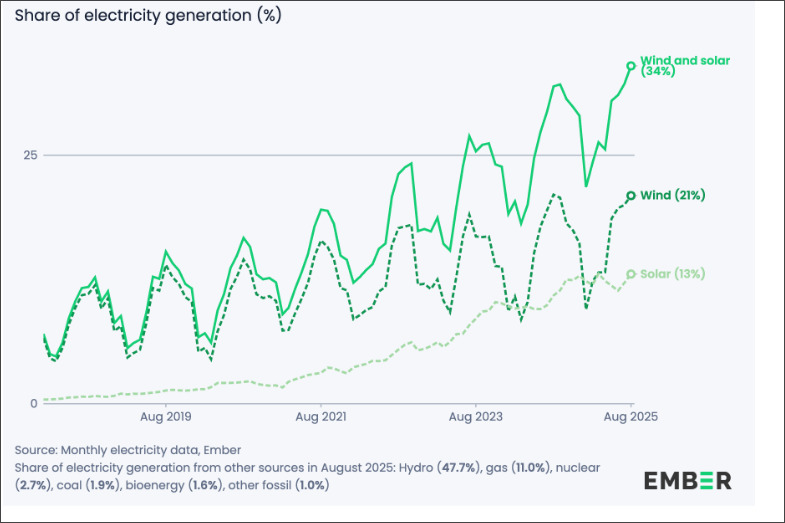
\includegraphics[width=0.9\textwidth]{grafico_ember.png}
            \caption{\footnotesize Geração Elétrica Renovável no Brasil (Ember, 2024).}
        \end{figure}
    \end{columns}
\end{frame}

\section{Problemática}

\begin{frame}{O Problema: Acúmulo de Poeira (\textit{Soiling})}
    \begin{columns}
        \column{0.5\textwidth}
        \begin{itemize}
            \item \textbf{Perdas de Eficiência:} Redução de até \textbf{7,84\% por semana} (Qi et al., 2025).
            \item \textbf{Cenários Críticos:} Perdas superiores a \textbf{50\%} em períodos de seca prolongada.
            \item \textbf{Efeito Físico:} Sombreamento das células e obstrução da radiação solar direta.
        \end{itemize}
        \column{0.5\textwidth}
        \begin{figure}
            \centering
            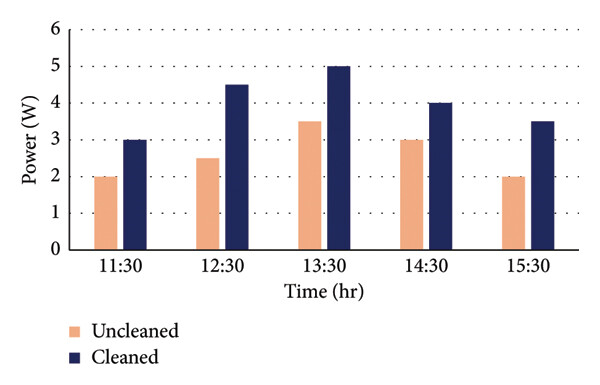
\includegraphics[width=0.9\textwidth]{grafico_soiling.jpg}
            \caption{\footnotesize Estudo sobre o impacto do \textit{soiling}. GEETHA, A. et al. (2025)}
        \end{figure}
    \end{columns}
\end{frame}

\begin{frame}{O Problema: Impacto Térmico}
    \begin{columns}
        \column{1\textwidth}
        \begin{itemize}
            \item \textbf{Coeficiente de Temperatura:} Decréscimo de \textbf{0,5\% a 0,6\%} por $^\circ$C acima de 25$^\circ$C.
            \item \textbf{Efeito Cumulativo:} Poeira retém calor na superfície.
            \item \textbf{Necessidade:} Sistema integrado de limpeza + \textit{cooling}.
        \end{itemize}
    \end{columns}
\end{frame}

\section{Estado da Arte}

\begin{frame}{Revisão Bibliográfica: Métodos de Limpeza}
    \begin{table}[]
        \centering
        \footnotesize
        \begin{tabular}{@{}lll@{}}
        \toprule
        \textbf{Método} & \textbf{Vantagens} & \textbf{Desvantagens} \\ \midrule
        \textbf{Robótica Autônoma} & Alta eficácia, sem água & Custo elevado, manutenção complexa \\
        \textbf{Revestimentos Nano} & Passivo, repele água & Custo proibitivo, baixa durabilidade \\
        \textbf{Aspersão + Wiper (ASCM)} & \textbf{Baixo custo, alta eficácia} & Consumo de água (se não gerido) \\ \bottomrule
        \end{tabular}
    \end{table}
    \begin{block}{Justificativa Técnica}
        Estudos de Geetha et al. (2024) demonstraram um aumento de \textbf{14,81\%} na eficiência utilizando o método de aspersão com rodo mecânico.
    \end{block}
\end{frame}

\begin{frame}{O Fenômeno de \textit{Dust Scaling}}
    \begin{itemize}
        \item \textbf{Formação de "Crosta":} A umidade (orvalho) cristaliza minerais solúveis entre as partículas de poeira e o vidro.
        \item \textbf{Adesão:} Cria-se uma camada rígida (\textit{hard scale}) difícil de remover apenas com ar.
        \item \textbf{Solução Integrada:} Uso otimizado de água para dissolver a crosta e ação mecânica para a remoção completa.
    \end{itemize}
\end{frame}

% --- Corpo do Projeto ---

\section{Objetivo Geral}
\begin{frame}{Objetivo Geral}
    \begin{block}{O que se espera do protótipo?}
        Desenvolver um protótipo de sistema automatizado de \textbf{baixo custo} para:
        \begin{itemize}
            \item \textbf{Limpeza Mecânica:} Remoção de poeira e detritos (\textit{soiling}).
            \item \textbf{Arrefecimento Térmico:} Controle de temperatura da superfície.
            \item \textbf{Sensoriamento em Tempo Real:} Monitoramento de potência e condições ambientais.
            \item \textbf{Gestão Hídrica:} Uso racional de água com potencial de reaproveitamento.
        \end{itemize}
    \end{block}
\end{frame}

\section{Materiais}
\begin{frame}{Materiais - Detalhamento de Componentes}
    \begin{columns}
        \column{0.5\textwidth}
        \textbf{Eletrônica e Controle:}
        \begin{itemize}
            \item Microcontrolador: Arduino Uno.
            \item Sensores de Corrente: INA219.
            \item Sensor de Temperatura: Termopar Impermeável.
            \item Driver de Motor: Ponte H L298N.
            \item Resistor de Carga (Potência).
        \end{itemize}

        \column{0.5\textwidth}
        \textbf{Mecânica e Estrutura:}
        \begin{itemize}
            \item Motores: DC com Redução.
            \item Atuadores Hídricos: Mini-bomba 12V e bicos aspersores.
            \item Estrutura: Peças em Impressão 3D.
        \end{itemize}
    \end{columns}
\end{frame}

\section{Metodologia}
\subsection{Hardware}
\begin{frame}{Metodologia - Hardware}
    \begin{itemize}
        \item \textbf{Arquitetura:} Integração de sensores para feedback em malha fechada.
        \item \textbf{Acionamento:} Sistema de movimentação linear para o rodo (\textit{wiper}).
    \end{itemize}
\end{frame}

\subsection{Software}
\begin{frame}{Metodologia - Software (Design 3D e Firmware)}
    \begin{itemize}
        \item \textbf{Modelagem 3D:} Utilização do software \textbf{Inventor} para design mecânico e simulação de movimentos.
        \item \textbf{Desenvolvimento de Firmware:} Linguagem C++/Arduino para lógica de controle.
        \item \textbf{Dashboard:} Interface simples para monitoramento e configuração de parâmetros via \textbf{Python}.
    \end{itemize}
\end{frame}

\subsection{Ferramentas de Execução}
\begin{frame}{Metodologia - Ferramentas de Execução}
    \begin{itemize}
        \item \textbf{Prototipagem Rápida:} Impressão 3D (FDM) para peças personalizadas.
        \item \textbf{Ambiente de Programação:} VS Code + Arduino IDE.
        \item \textbf{Instrumentação:} Multímetro e protoboards para validação de circuitos.
    \end{itemize}
\end{frame}

\section{Cronograma}

\begin{frame}{Cronograma Detalhado (Parte 1: Março e Abril)}
    \centering
    \scriptsize
    \begin{tabular}{|l|c|c|c|c|c|c|c|c|c|}
    \hline
    \textbf{Atividade / Semana} & \textbf{S1} & \textbf{S2} & \textbf{S3} & \textbf{S4} & \textbf{S5} & \textbf{S6} & \textbf{S7} & \textbf{S8} & \textbf{S9} \\ \hline
    \textit{Datas (Início da Sem.)} & \tiny 03/03 & \tiny 10/03 & \tiny 17/03 & \tiny 24/03 & \tiny 31/03 & \tiny 07/04 & \tiny 14/04 & \tiny 21/04 & \tiny 28/04 \\ \hline
    Revisão Bibliográfica & X & X & X & & & & & & \\ \hline
    Definição/Compra Materiais & & X & X & X & X & X & & & \\ \hline
    \textbf{Design 3D (Inventor)} & & & & & \cellcolor{blue!20}X & \cellcolor{blue!20}X & \cellcolor{blue!20}X & & \\ \hline
    \textbf{Programação (Firmware)} & & & & & \cellcolor{blue!20}X & \cellcolor{blue!20}X & \cellcolor{blue!20}X & \cellcolor{blue!20}X & \cellcolor{blue!20}X \\ \hline
    Escrita do Artigo & & & & & & & \cellcolor{yellow!20}X & \cellcolor{yellow!20}X & \cellcolor{yellow!20}X \\ \hline
    \end{tabular}
\end{frame}

\begin{frame}{Cronograma Detalhado (Parte 2: Maio a Junho)}
    \centering
    \scriptsize
    \begin{tabular}{|l|c|c|c|c|c|c|c|c|}
    \hline
    \textbf{Atividade / Semana} & \textbf{S10} & \textbf{S11} & \textbf{S12} & \textbf{S13} & \textbf{S14} & \textbf{S15} & \textbf{S16} & \textbf{S17} \\ \hline
    \textit{Datas (Início da Sem.)} & \tiny 05/05 & \tiny 12/05 & \tiny 19/05 & \tiny 26/05 & \tiny 02/06 & \tiny 09/06 & \tiny 16/06 & \tiny 23/06 \\ \hline
    Montagem Mecânica/Eletrônica & X & X & X & & & & & \\ \hline
    Refino de Software & X & X & X & X & & & & \\ \hline
    Testes e Validação & & & & X & X & X & X & \\ \hline
    Finalização do Artigo & & & & & X & X & X & \cellcolor{red!20}\textbf{FIM} \\ \hline
    \end{tabular}
\end{frame}

\section{Bibliografia}
\begin{frame}{Bibliografia Selecionada}
    \footnotesize
    \begin{itemize}
        \item \textbf{GEETHA, A. et al.} Solar Panel Self-Cleaning Mechanisms and Its Effect on the Economic and Environmental Sustainability. Journal of Electrical and Computer Engineering, 2024.
        \item \textbf{QI, J. et al.} Combining dust scaling behaviors of PV panels and water cleaning methods. Renewable and Sustainable Energy Reviews, 2025.
        \item \textbf{CAVALCANTE, M. M. et al.} Protótipo de um sistema automatizado para higienização de painéis solares... Anais do V SINGEP, 2016.
        \item \textbf{EMBER.} European Electricity Review 2026 \& Brazil Wind/Solar Report 2024.
    \end{itemize}
\end{frame}

\end{document}
